%! Author = jay
%! Date = 10/25/24

% Preamble
\documentclass[11pt]{beamer}
\usetheme{JuanLesPins}
\usecolortheme{dolphin}

% Packages
\usepackage{amsmath}
\usepackage{tikz}
\usepackage[outputdir=../out]{minted}
\usepackage{pgfplots}
\usepackage{pgf}
\usepackage{lmodern}
\usepackage{blkarray}

\def\mathdefault#1{#1}
\everymath=\expandafter{\the\everymath\displaystyle}
\makeatletter\@ifpackageloaded{underscore}{}{\usepackage[strings]{underscore}
\usepackage{listings}}\makeatother

\pgfplotsset{compat=1.17}
\usetikzlibrary{arrows.meta} %define styles in graph

\usepgfplotslibrary{external}
\tikzexternalize

\setminted{fontsize=\small}

\title{GPU Programming: Rather Feasible}

% Document
\begin{document}
    \newcommand{\mkAgenda}{
    \begin{frame}{Outline}
        \tableofcontents[currentsection]
    \end{frame}
}

\newcommand{\CUDA}[1]{{\mintinline[breaklines,breakafter=,]{CUDA}{#1}}}

\newcommand{\slide}[3]{
    \begin{frame}{#1}
        \center
        \begin{columns}
            \begin{column}{0.35\textwidth}
                \center
                \begin{itemize}
                    #2
                \end{itemize}
            \end{column}
            \begin{column}{0.6\textwidth}
                \begin{center}
                    #3
                \end{center}
            \end{column}
        \end{columns}
    \end{frame}
}

\newcommand{\append}[1]{
    \begin{minipage}[c]{0.66\linewidth}
    \resizebox{\textwidth}{!}{\input{#1}}
    \end{minipage}
}

\newcommand{\appendTwo}[2]{
    \begin{minipage}[c]{0.45\linewidth}
        \resizebox{\textwidth}{!}{\input{#1}}
    \end{minipage}
    \begin{minipage}[c]{0.45\linewidth}
        \resizebox{\textwidth}{!}{\input{#2}}
    \end{minipage}
}

\newcommand{\true}{TRUE}
\newcommand{\false}{FALSE}

\newcommand{\sectionSlide}[1]{
    \begin{frame}
      \vfill
      \centering
      \begin{beamercolorbox}[sep=8pt,center,shadow=true,rounded=true]{title}
        \usebeamerfont{title}\insertsectionhead\par%
      \end{beamercolorbox}
      \ifx#1\true{\tableofcontents[currentsection]}\fi
      \vfill
  \end{frame}
}

    \begin{frame}
        \titlepage
    \end{frame}

    \begin{frame}{Outline}
        \tableofcontents
    \end{frame}

    \section{CUDA?}\label{sec:cuda?}
\mkAgenda

\begin{frame}{CUDA?}
    \center
    \begin{itemize}
        \item<1-> nVidia 2007
        \item<2-> GPGPU
    \end{itemize}

    \begin{columns}
        \begin{column}{0.4\textwidth}
            \begin{itemize} \item<3-> Platform/language \end{itemize}
        \end{column}
        \begin{column}{0.4\textwidth}
            \begin{itemize} \item<3-> API/library \end{itemize}
        \end{column}
    \end{columns}

    \begin{columns}
        \begin{column}{0.4\textwidth}
            \begin{itemize}
                \item[]<4-> C++
                \item[+]<5-> keywords {\CUDA{__host__ __device__}}
                \item[+]<6-> syntax {\CUDA{kernel<<<blk, thrd>>>()}}
            \end{itemize}
        \end{column}

        \begin{column}{0.4\textwidth}
            \begin{itemize}
                \item[]<7-> {\CUDA{cudaMalloc}}
                \item[]<7-> {\CUDA{cudaMemcpy}}
                \item[]<7-> {\CUDA{__syncthreads}}
                \item[]<7-> {\CUDA{threadIdx}}
            \end{itemize}
        \end{column}
    \end{columns}
\end{frame}
    \section{Rationale}\label{sec:rationale}
\mkAgenda

\begin{frame}[fragile]{Rationale}
    \center
    \begin{minted}[linenos,breaklines=true]{CUDA}
for(size_t i = 0; i < m; i++) {
  for(size_t j = 0; j < p; j++) {
    c[i * p + j] = 0;
    for(size_t k = 0; k < n; k++) {
      c[i * p + j] += a[i * n + k] * b[k * p + j];
    }
  }
}
    \end{minted}
\end{frame}

\begin{frame}{Rationale}
    \center
    \appendTwo{./figures/time.pgf}{./figures/elems.pgf}
\end{frame}
    \section{Thinking in GPUs}\label{sec:thinking-in-gpus}
\mkAgenda

\begin{frame}{Thinking in GPUs}
    \center
    \begin{itemize}
        \item<1-> Threads \textrightarrow Warps \textrightarrow SMs \textrightarrow GPU
    \end{itemize}
    \onslide<2->{
        \begin{block}{Branches}
            \begin{itemize}
                \item Warps use SIMT \textrightarrow all threads run same instruction
            \end{itemize}
        \end{block}
    }
    \onslide<3->{
        \begin{block}{Memory}
            \begin{itemize}
                \item Unified memory: \CUDA{cudaMallocManaged} (CUDA 4+)
                \begin{itemize}
                    \item<4-> Automatic page migration
                    \item<4-> Up to GeForce 9XX: slow
                    \item<4-> Starting with GeForce GTX 10XX (CUDA 6+): GPU page faults increase performance
                \end{itemize}
                \item Separate address spaces: \CUDA{cudaMalloc}
                \begin{itemize}
                    \item<5-> Requires manual \CUDA{cudaMemcpy}
                \end{itemize}
                \item<6-> \CUDA{cudaFree} to clean up
            \end{itemize}
        \end{block}
    }
\end{frame}
    \section{Example}\label{sec:example}
\mkAgenda

\begin{frame}[fragile]{Example (C++)}
    \center
    \begin{minted}[linenos,breaklines=true]{C++}
void matmul_cpu(float *a, float *b, float *c, size_t m, size_t n, size_t p) {
  for(size_t i = 0; i < m; i++) {
    for(size_t j = 0; j < p; j++) {
      c[i * p + j] = 0;
      for(size_t k = 0; k < n; k++) {
        c[i * p + j] += a[i * n + k] * b[k * p + j];
      }
    }
  }
}
// ...
matmul_cpu(a, b, c, m, n, p);
    \end{minted}
\end{frame}

\begin{frame}[fragile]{Example (C++)}
    \center
    \begin{itemize}
        \item<1-> $\mathcal{O}(m \cdot n \cdot p)$ operations
        \item<2-> $m \cdot p$ independent (write different elements of \CUDA{c})
        \item<3-> Idea: launch $m \cdot p$ threads on GPU
    \end{itemize}
    \onslide<4->{
        \begin{block}{Synchronization}
            All threads should do independent work - synchronization is expensive!
        \end{block}
    }
\end{frame}

\subsection{Preparation}\label{subsec:preparation}
\begin{frame}[fragile]{Preparation}
    \center
    \begin{minted}[linenos,breaklines=true]{C++}
float *a, *b, *c;
size_t m, n, p;
// ... data is readied here ...
    \end{minted}
\end{frame}

\begin{frame}[fragile]{Preparation}
    \center
    Separate address spaces $\Rightarrow$ ready memory
    \begin{minted}[linenos,firstnumber=4,breaklines=true]{C++}
// create buffers on GPU ...
float *a_dev, *b_dev, *c_dev;
cudaMalloc(&a_dev, m * n * sizeof(float));
cudaMalloc(&b_dev, n * p * sizeof(float));
cudaMalloc(&c_dev, m * p * sizeof(float));
// ... and copy relevant data
cudaMemcpy(a_dev, a, m * n * sizeof(float), cudaMemcpyDefault);
cudaMemcpy(b_dev, b, n * p * sizeof(float), cudaMemcpyDefault);

// TODO: start GPU threads
    \end{minted}
\end{frame}

\begin{frame}[fragile]{Preparation}
    \center
    After GPU finishes, copy data back
    \begin{minted}[linenos,firstnumber=13,breaklines=true]{CUDA}
// TODO: start GPU threads

cudaMemcpy(c, c_dev, m * p * sizeof(float), cudaMemcpyDefault);
    \end{minted}
\end{frame}

\subsection{Kernel}\label{subsec:kernel}
\begin{frame}[fragile]{Kernel}
    \center
    \begin{itemize}
        \item<1-> Each function: execution space
        \item<2-> Three possible:
        \begin{itemize}
            \item<2-> \CUDA{__host__}: CPU only
            \item<2-> \CUDA{__device__}: GPU only
            \item<2-> \CUDA{__global__}: CPU to GPU entry
            \item<3-> Can combine \CUDA{__host__ __device__}
        \end{itemize}
    \end{itemize}
    \onslide<4->{
        \begin{block}{\CUDA{__global__}}
            Functions marked as \CUDA{__global__} should always be \CUDA{void}
        \end{block}
    }
\end{frame}

\begin{frame}[fragile]{Kernel}
    \center
    \begin{minted}[linenos,breaklines=true]{CUDA}
__global__ void matmul_gpu(float *a, float *b, float *c, size_t m, size_t n, size_t p) {
  size_t i = some_magic_trick();
  size_t j = some_other_magic_trick();
  c[i * p + j] = 0;
  for(size_t k = 0; k < n; k++) {
    c[i * p + j] += a[i * n + k] * b[k * p + j];
  }
}
    \end{minted}
    \begin{itemize}
        \item<2-> Notice keyword \CUDA{__global__}
        \item<3-> How to get \CUDA{i}, \CUDA{j}?
    \end{itemize}
\end{frame}

\begin{frame}[fragile]{Kernel}
    \center
    \begin{itemize}
        \item<1-> \CUDA{i}, \CUDA{j}? \textrightarrow use thread index
        \item<2-> Threads are launched in blocks of threads
        \item<3-> Sizes are defined in 3D
        \item<4-> Preferably launch in powers of 2
    \end{itemize}
    \onslide<3->{
        \centerline{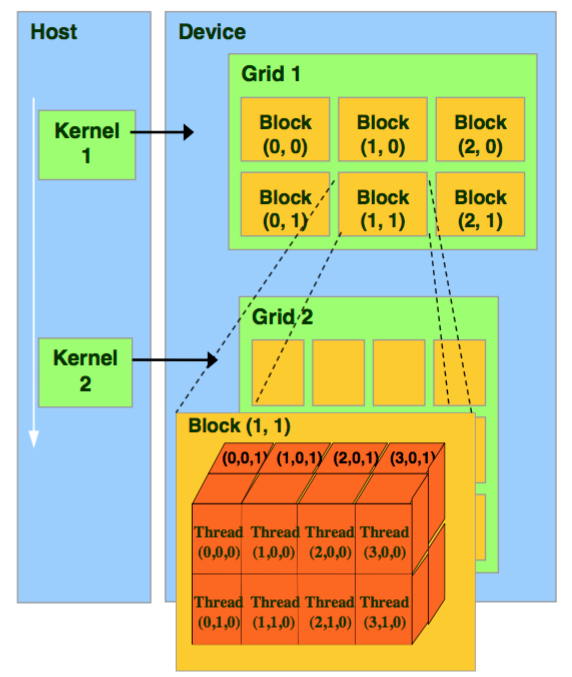
\includegraphics[width=0.33\textwidth]{./figures/thread-mapping}}
    }
\end{frame}

\begin{frame}[fragile]{Kernel}
    \center
    \begin{minted}[linenos,breaklines=true]{CUDA}
__global__ void matmul_gpu(float *a, float *b, float *c, size_t m, size_t n, size_t p) {
  size_t i = threadIdx.x + blockIdx.x * blockDim.x;
  size_t j = threadIdx.y + blockIdx.y * blockDim.y;
  if(i >= m || j >= p) return; // out of bounds
  c[i * p + j] = 0;
  for(size_t k = 0; k < n; k++) {
    c[i * p + j] += a[i * n + k] * b[k * p + j];
  }
}
    \end{minted}
\end{frame}

\subsection{Launch}\label{subsec:launch}
\begin{frame}[fragile]{Launch}
    \center
    \begin{itemize}
        \item<1-> Kernel launch using special syntax \CUDA{<<<>>>}
    \end{itemize}
    \onslide<2->{\centerline{\CUDA{matmul_gpu<<<blocks, threads>>>(args)}}}
    \begin{itemize}
        \item<3-> \CUDA{blocks} and \CUDA{threads} are \CUDA{dim3} values
        \item<4-> \CUDA{dim3(x)}, \CUDA{dim3(x, y)}, \CUDA{dim3(x, y, z)} are all valid
        \item<5-> Arguments are passed as normal
        \item<6-> Launch is asynchronous; wait for completion using \CUDA{cudaDeviceSynchronize()}
    \end{itemize}
\end{frame}

\begin{frame}[fragile]{Launch}
    \center
    \begin{minted}[linenos,firstnumber=10,breaklines=true]{CUDA}
// ...
cudaMemcpy(a_dev, a, m * n * sizeof(float), cudaMemcpyDefault);
cudaMemcpy(b_dev, b, n * p * sizeof(float), cudaMemcpyDefault);

auto blocks = dim3(m / 1024 + 1, p / 1024 + 1);
auto threads = dim3(1024, 1024);
matmul_gpu<<<blocks, threads>>>(a_dev, b_dev, c_dev, m, n, p);
cudaDeviceSynchronize(); // wait for GPU to finish

cudaMemcpy(c, c_dev, m * p * sizeof(float), cudaMemcpyDefault);
    \end{minted}
\end{frame}

    \section{Extras}\label{sec:extras}
\mkAgenda

\subsection{Errors}\label{subsec:errors}
\begin{frame}[fragile]{Errors}
    \center
    \begin{itemize}
        \item<1-> CUDA functions return \CUDA{cudaError_t}, useful with \CUDA{cudaGetErrorString()}
    \end{itemize}
\begin{minted}[breaklines=true]{CUDA}
#define CHECK(x) do { \
    const auto _ = (x); \
    if(_ != cudaSuccess) { \
        /* ... handle error using cudaGetErrorString(_) */\
    } \
} while(false)
\end{minted}
\end{frame}

\subsection{Memory}\label{subsec:memory}
\begin{frame}{Memory}
    \center
    \begin{itemize}
        \item Manage GPU memory
        \item Allocate with \CUDA{cudaMalloc(void **dev, size_t bytes)}
        \item Read/Write CPU-side with \CUDA{cudaMemcpy(void *dst, const void *src, size_t bytes, cudaMemcpyKind kind)}
        \begin{itemize}
            \item \CUDA{cudaMemcpyDefault}: Inferred based on pointers (CUDA 4+)
            \item \CUDA{cudaMemcpyHostToDevice}: CPU \textrightarrow GPU
            \item \CUDA{cudaMemcpyDeviceToHost}: GPU \textrightarrow CPU
            \item \CUDA{cudaMemcpyDeviceToDevice}: GPU \textrightarrow GPU
            \item \CUDA{cudaMemcpyHostToHost}: CPU \textrightarrow CPU
        \end{itemize}
        \item Unified Memory: \CUDA{cudaMallocManaged(void **dev, size_t bytes)} (accessible on CPU \& GPU)
        \item Free/Clean up with \CUDA{cudaFree(void *dev)}
    \end{itemize}
\end{frame}

\subsection{Synchronization}\label{subsec:synchronization}
\begin{frame}[fragile]{Synchronization}
    \center
    \begin{itemize}
        \item Atomic functions like \CUDA{atomicAdd}
        \item Across threads/warps in block: \CUDA{__syncthreads()}
        \item Make CPU wait for GPU: \CUDA{cudaDeviceSynchronize()}
        \item More advanced:
        \begin{itemize}
            \item Selected threads using \CUDA{cuda::barrier}
            \item All threads across blocks: \CUDA{this_grid().sync()} (requires Cooperative Groups and launch using \CUDA{cudaLaunchCooperativeKernel})
        \end{itemize}
    \end{itemize}
\end{frame}

\subsection{CUDA $\leftrightarrow$ OpenGL}\label{subsec:cuda-opengl}
\begin{frame}[fragile]{CUDA $\leftrightarrow$ OpenGL}
    \center
    \begin{itemize}
        \item<1-> \CUDA{__device__} functions can access OpenGL data
    \end{itemize}
    \begin{minted}[breaklines=true]{CUDA}
#include <cuda_gl_interop.h>
// set up on CPU
cudaGraphicsResource *resource; T *dev_ptr; size_t size;
cudaGraphicsGLRegisterBuffer(&resource, handle, cudaGraphicsRegisterFlagsNone);
cudaGraphicsMapResources(1, &resource);
cudaGraphicsResourceGetMappedPointer(
    reinterpret_cast<void **>(&dev_ptr), &size, resource
);
// ... do stuff with dev_ptr on GPU
// clean up on CPU
cudaGraphicsUnmapResources(1, &resource);
cudaGraphicsUnregisterResource(resource);
    \end{minted}
\end{frame}

\end{document}

% CUDA???                               CHECK
% Rationale                             CHECK
% Getting Started                       CHECK
% - Basics: host vs device, memory
% - Thinking in GPUs
% Example                               CHECK
% - CPU program
% - ... conversion
% - CUDA program
% Nice to knows/Reference